\documentclass[11pt,a4paper,titlepage]{report}

\usepackage{url}
\usepackage{csquotes}
\usepackage[backend=biber, style=trad-abbrv]{biblatex}
\usepackage{amsmath}
\usepackage{amssymb}
\usepackage{graphicx}
\usepackage{siunitx}
\usepackage{listings}
\usepackage{titling}
\newcommand{\subtitle}[1]{%
	\posttitle{%
		\par\end{center}
	\begin{center}\large#1\end{center}
	\vskip0.5em}%
}
\lstset{
	frame=tb,
	language=c,
	aboveskip=3mm,
	belowskip=3mm,
	showstringspaces=false,
	columns=flexible,
	basicstyle={\small\ttfamily},
	numbers=left,
	breaklines=true,
	breakatwhitespace=true,
	tabsize=3
}

\title{Final Project}
\subtitle{Autonomous Underwater Vehicle}
\author{Richard Sefton}

\graphicspath{./assets/}
\usepackage[inkscapeformat=png]{svg}

\addbibresource{BIBLIOGRAPHY.bib}

\setcounter{chapter}{1}

\begin{document}
	\maketitle
	\tableofcontents
	
	\begin{abstract}
		This report depicts the end to end design and development of an Autonomous Underwater Vehicle for the Final Project of the BSc Computer Science degree. As it transpires this was an incredibly ambitious project to deliver in such a short time frame. This report will try to capture the key aspects of the development process which will be a challenge in itself given the constraints on the report and as such, some aspects will be focused on more than others.  
	\end{abstract}
	
	\chapter*{Introduction} (max 2 pages)
	\addcontentsline{toc}{chapter}{Introduction}
	Autonomous Underwater Vehicles have been around since the 1950s, with the first AUV on record developed by Washington University in 1957 named SPURV\cite{SPURV} (Self Propelled Underwater Research Vehicle). The device was fitted with various temperature and pressure sending probes and could traverse to depths of 3600\unit{\meter} and one of the last uses of the SPURV AUV was to study submarine wakes in the 70s. Since this first development, in the last 67 years AUVs have been refined and further developed by various governments, oceanographic institutes, universities and private companies. Today, AUVs are often considered cheaper, better and safer to deploy than manned underwater vehicles (particularly in the light of the more recent Titan submarine implosion\cite{TITAN_IMPLOSION}), and safer than deploying divers. They are capable of obtaining more data than any single diver can obtain, and capable of diving longer than any manned vehicle as the requirement for breathable air is negated. An AUVs dive time is only limited by its available power which will only increase as power technology improves. AUVs are used across a multitude of different industrial sectors spanning scientific research, surveying, military, shipping and gas and oil\cite{AUV_MARKETSHARE}. 
	
	The aim of this project is to design and develop a rudimentary AUV. This project does not comfortably fall into any of the predefined template project ideas but was born from a personal enjoyment of the Internet of Things module which allowed me to explore microcontroller programming and interacting with physical sensors and actuators, which blossomed into a passion for robotics. As one of the early module videos highlighted, our projects should be something we are passionate about as without passion we would lack the motivation to complete such a lengthy and isolated piece of work\cite{COURSERA_PROJECT_VIDEO}. I found that the existing Internet of Things templates involved topics I'm not particularly passionate about. I did gain permission from the Coursera Tutor Forums prior to embarking on this journey\cite{COURSERA_PROJECT_PERMISSION}.
	
	This project was initially inspired by the work of a YouTuber (Brick Experiment Channel\cite{BRICK_EXPERIMENT_CHANNEL_PROFILE}) who created a small remote controlled submarine using a watertight container and Lego. The accompanying blog\cite{BRICK_EXPERIMENT_CHANNEL_BLOG} depicts the design and development of several versions of this device, and also explains some of the key concepts that need to be considered such as buoyancy. The original plan for this project was to do something similar to this (occupying the hobby space of the AUV market) - a small device that provides basic functionality autonomously, using similar materials (a water tight container and Lego). However, following the initial research into the AUV market there is a trend of AUVs costing thousands\cite{AUV_COST}, a cost which will increase with the additional custom payloads (sensor arrays) required for the specific research projects. There are a small handful of manufacturers that offer lower cost AUVs to customers such as the ecoSub\cite{ECOSUB} which states one of their submarines are \unit{\approx}£15k, this is a price point that may still be out of reach for many projects. In addition to the initial cost of AUVs being expensive, the parts would be custom made by the manufacturer and so any repairs could be equally costly. 
	
	While the inspiration for this project started with a small remote controlled submarine, the initial research has expanded the scope to try and develop an extremely low cost AUV which could be made open source (allowing for easy customisations) and can be manufactured by the researchers that require them using readily available parts and 3D printing which is now common relatively common and would mitigate the requirement for $3^{rd}$ party companies fabricating parts. This would also mitigate costly repairs as all the design files would be a part of the project. The target users of this AUV may be required to develop their own payloads, but even the cost of hiring a developer to do this may still be cheaper than buying AUVs from known sources. 
	
	By developing an open source AUV, this could seriously open up underwater research for projects that are underfunded. These projects may have previously relied on human divers to obtain data as the safer unmanned alternative is out of reach for them so this would make such endeavours safer too.  
	
	\chapter*{Literature Review} (max 5 pages)
	\addcontentsline{toc}{chapter}{Literature Review}
	\section*{Previous works}
	\addcontentsline{toc}{section}{Previous Works}
	\subsection*{Amateur Level}
	\addcontentsline{toc}{subsection}{Amateur Level}
	The YouTuber Brick Experiment Channel\cite{BRICK_EXPERIMENT_CHANNEL_PROFILE} wrote a series of blog posts\cite{BRICK_EXPERIMENT_CHANNEL_BLOG} outlining the build process for the $4^{th}$ iteration of their remote controlled submarine. 
	
	The posts are detailed covering the steps of building this submarine with reasoning behind the design decisions along with a critical evaluation of each step. This version is using a large syringe to bring water onboard the vehicle to control buoyancy, and is driven by two motors: one for propulsion, and one for direction. The sensors incorporated measure pressure to accurately gauge depth, and a laser to measure distance from the bed of a body of water. 
	
	The blog also raised communication as a consideration: While the aim of this project is to build an autonomous vehicle, it would be nice to communicate with it in flight. The problem is this cannot be done easily with wireless frequencies as the higher frequencies that provide the required bandwidth do not penetrate water that well.
	
	\subsection*{Commercial Level}
	\addcontentsline{toc}{subsection}{Commercial Level}
	The company Advanced Navigation makes the Hydrus Drone\cite{ADVANCED_NAVIGATION_HYDRUS}, which claims to be one of the smallest AUVs on the market. The device itself controls depth and position with impellers, a 4K camera with AI integrations, and a forward facing sonar. The most important aspect of Advanced Navigation's AUV is how they address the issues around wireless communication. This company has fitted their device with acoustic and optical modems so data can be transferred using audio frequencies and light (presumably similar to fibre octics).
	
	\subsection*{Research Level}
	\addcontentsline{toc}{subsection}{Research Level}
	The Woods Hole Oceanographic Institute\cite{WOODS_HOLE} draws attention to the use of different AUVs depending on the area of research or environment. They use one of 6 AUV models, which operate at different depths or different functionality. The REMUS\cite{WOODS_HOLE_REMUS} can be equipped with varying sensors and is programmed for survey missions. It was also adapted to survey the Delaware river Aqueduct for leaks. 
	
	One of the more interesting AUVs this institute uses is the Spray Glider\cite{WOODS_HOLE_SPRAY_GLIDER}. This description for this device is one that glides through the water without any external thrusters so can be travel for weeks at a time. The device uses internal bladders to control buoyancy, and is set to navigate preset paths equipped with varying sensors. What is interesting about this device is the lack of external propulsion seems to make this device more passive, and can therefore operate at lower voltage.
	
	The UK National Oceanography Centre has details on the challenges around an designing an AUV\cite{NATIONAL_OCEANOGRAPHIC_AUTOSUBS}. For power and propulsion it highlights the lack of oxygen for internal combustion makes it necessary to use batteries for power and notes the difference in speed between AUVs and surface ships. For navigation it highlights that because GPS can't penetrate the top few mm of water, the reliance on other techniques is required. It suggests an approach called Dead Reckoning which gets the speed of the AUV by measuring the Doppler shift from the sea bed for relative speed and using a gyro to measure the heading. It highlights that navigational accuracy is vital to survey missions. 
	
	\section*{Key Literature}
	\addcontentsline{toc}{chapter}{Key Literature}
	The definition for an AUV is best described in an article titled ``Autonomous Underwater Vehicles (AUVs): Their past, present and future contributions to the advancement of marine geoscience". 
	
	\begin{quote}
		Autonomous Underwater Vehicles (AUVs) are unmanned, self-propelled vehicles that are typically deployed from a surface vessel, and can operate independently of that vessel for periods of a few h to several days.\cite{AUV_PPF}
	\end{quote}
	
	The authors go on to highlight that ``In addition, recent economic drivers, such as rapidly increasing vessel fuel oil costs, are making autonomous systems a potentially attractive proposition to organisations responsible for large-scale and cost-effective marine data collection programmes"\cite{AUV_PPF}. This article addresses the commercial benefits of AUV production and deployment but doesn't address the human benefits such as safety. 
	
	The authors also discuss the applications of AUVs and point out that ``the sensors deployed determine the vehicle altitude, as well as its speed and endurance."\cite{AUV_PPF} The endurance in this context is the available power to the AUV which would affect its overall range. Because different sensors and actuators have varying power requirements, some of these components may draw more power than others. The array of sensors required is defined by the AUVs use case: it would be inefficient mounting water quality sensors onto an AUV designed for ocean bed mapping survey. 
	
	While this article includes a lot of jargon relating to marine geosciences, it provides a good overview of the uses of AUVs and their previous applications. More importantly, it provides some good starting points for some concepts I will need to  explore during the development of this project. This includes references to works that look into the Dead Reckoning method of positioning, and a launch pad into some key concepts such as Sonar. 

	Because the sensors deployed on an AUV are specific to its function and is something that can be configured, it is worth considering a modular design. As a part of this there could be some level of connectivity between the separate modules. Modern MCUs typically feature multiple options for communication protocols such as UART, USART, $I^{2}C$, SPI, USB, Ethernet or could be as simple as pulling a pin high or low. For the purpose of this project, we will consider $I^{2}C$ as it uses minimal wires, and allows for two way communication. The MCU data sheet\cite{ATTINY1627} is the manufacturers documentation and is a vital reference for development on any given  MCU and it directly relates to the MCU specific library in code. It has all the details and requirements to setup any of the provided MCU features, and gives a brief overview of each feature. 
	
	With regards to the ATTiny 1627 MCU, the data sheet describes $I^{2}C$ as a TWI (Two Wire Interface): ``The Two-Wire Interface (TWI) is a bidirectional, two-wire communication interface (bus) with a Serial Data Line (SDA) and a Serial Clock Line (SCL)"\cite{ATTINY1627}. There are several advantages to using the TWI bus as a communication protocol as it allows the connection of ``one or several slave devices to one or several master devices"\cite{ATTINY1627} allowing a network of devices to become interconnected. This would also allow for parallel computation as instead leaving one device to perform all of the sensor readings and calculations, some of which could be computationally expensive or using deliberate pauses of code execution, a master device could simply trigger the networked modules to each perform their actions and then do nothing while waiting for the responses. 
	
	In the article 'FEATURES, OPERATION PRINCIPLE AND LIMITS OF SPI AND $I^{2}C$ COMMUNICATION PROTOCOLS FOR SMART OBJECTS' the authors share their opinion on how an IoT network should operate and how it should be secured, and then give an overview of both $I^{2}C$ and SPI protocols before suggesting a hybrid version of the two. For IoT networks the authors suggest that ``different devices with different capabilities will take part in the creation of a network. A self-describing interface for each device is necessary in order to optimize the management of required tasks"\cite{I2C}. This point backs up my idea of a modular design where sensor modules can be attached in a way to form a network where each module is responsible for a specific task. They then go on to highlight that ``adding an object to the network should not cause the collapse of the network itself. The network should also properly handle the failure of a device"\cite{I2C}. This point involves error handling within a network of discreet modules. If one module fails, the whole unit should not. If the module is deemed vital to the devices operation, such as obstacle avoidance sensors on an AUV, a graceful way to handle this could be to surface the device and broadcast a signal indicating the error on a predefined wavelength so it can be collected. 
	
	For $I^{2}C$ the authors give a detailed overview stating that:
	
	\begin{quote}
		The \textit{Inter Integrated Circuit} ($I^{2}C$) protocol, ..., was developed by Philips in 1982 and it is a serial, single-ended bus with multi-master support and typically used to connect low speed devices.\cite{I2C}
	\end{quote}
	
	The bandwidth available over the standard $I^{2}C$ rail is slow at 100\unit{\kilo\bit}/\unit{\second}, but there is a Fast mode and Fast Plus mode which allows up to 1\unit{\mega\bit}/\unit{\second}. Additionally some devices also support a high speed mode which allows up to 3.4\unit{\mega\bit}/\unit{\second}.\cite{I2C_FAST}. This means the $I^{2}C$ rail may not be suitable for \textit{all} types of sensors attached, particularly ones that gather a lot of data in real time, for example high definition cameras. 
	
	\begin{quote}
		Since the bus is completely shared, it is possible, for devices, to receive not only unicast transmission but also broadcast messages: for this reason, whenever master wants to write or read data from a particular slave, it will address it first. Addressing bits were originally seven, extended to 10 with the latest reviews to increase supported maximum number of connected devices. $I^{2}C$ bus supports multiple masters on the same bus too, but a proper conflict-solving algorithm has to be implemented. \cite{I2C}
	\end{quote}
	
	This addressing is how the devices know what devices they need to talk to on a network. With the system of addressing and the ability to broadcast transmissions we can begin to visualise the $I^{2}C$ protocol as akin to web sockets. The interesting point raised here is that conflict resolution needs to be handled where the network has multiple masters. One such proposal they put forward is Arbitration: ``since $I^{2}C$ supports multiple masters, an arbitration rule is necessary. In this protocol, arbitration proceeds bit by bit and the rule is deterministic: the first master that produces a one when the other produces a zero loses the arbitration"\cite{I2C}. 
	
	Another resource that covers a lot of information about AVR Microcontrollers and also providing an overview of the features as well as how to interact with actuators such as servos and stepper motors, is 'Make: AVR Programming'\cite{MAKE_AVR}. While this book does contain quite a broad overview of the features and protocols, it also has examples of code to interact with them, as well as an overview of the toolchain required to programme a microcontroller (in this instance involving Make, avr-gcc\cite{GCC_AVR} and AVRDude\cite{AVRDUDE} as well as a physical hardware programmer). However, the example code is all written for a specific MCU that the book focuses on, being the ATMEGA168. However, as the author notes, this should not be too difficult to port to my specifically chosen MCU as the book also tries to teach another skill being the ability to refer to relevant sections of the data sheet. 
	
	As well as internal device communication protocols, it would also be good if we could have some way of interacting with the device in flight: receiving data, and possibly some rudimentary manual over ride/remote control. As corroborated in an article exploring underwater wireless networks, ``radio is seriously attenuated in water"\cite{UNDERWATER_RADIO}. Radio waves exist on the EM Spectrum and the lower the frequency, the further it can penetrate water due to the electrical dissipation that occurs, which is accentuated by salt water. High frequencies that we are used to as standard data transfer frequencies (WiFi, Bluetooth) are measured in \unit{\giga\hertz}, and these penetrate only a few \unit{\centi\meter} of water. Even LoRa at 433\unit{\mega\hertz} will only penetrate 30-50\unit{\centi\meter} of water. The military use lower radio frequencies operating in the range of \unit{\hertz} to \unit{\kilo\hertz} to communicate with their submarines but the trade off is lower frequencies bandwidth (less data can be transferred as there are fewer cycles per second). Additionally, radio frequencies are controlled\cite{RADIO_FREQ_TABLE} and as a hobby enthusiast/student I only have access to a limited range of frequencies.  
	
	The article also states ``acoustic communication is almost the only effective way for underwater wireless transmission. Nevertheless, compared with the traditional radio, underwater acoustic communication is greatly affected by poor conditions, such as absorption, scattering, multipath interference and Doppler effect"\cite{UNDERWATER_RADIO}. While I think the authors are perhaps exaggerating this point to justify their experiments somewhat, it does offer an alternate avenue to wireless communication with a device while it is operating underwater, but it would require the development of an ultrasonic modem of some description. Alternatively we could just add a plug to the device for a physical wire for external control/data transmission. While this goes against the design of an AUV as being untethered, it would also act as a lifeline to retrieve the device while minimising risk, even when testing in controlled bodies of water.
	
	\chapter*{Design} (max 4 pages)
	\addcontentsline{toc}{chapter}{Project Design}
	\section*{Domain}
	\addcontentsline{toc}{section}{Domain}
	AUVs have applications spanning multiple domains both in scientific exploration as well as commercial enterprise. For science they are used for surveying coastlines and ocean beds, sampling in remote or hard to reach locations and exploring the depths to name a few applications. For commerce they can de deployed to monitor gas and oil pipelines, drills, survey potential resource sites, and monitor ship hulls etc. The deployment of AUVs over physical diving or manned equipment offer more benefits when compared to the cost and safety. AUVs can potentially spend longer underwater depending on the design and payload they are equipped with and the size of the power source, and can gather far more data than a diver with far less risk to human life.
	
	For this project, the aim was to develop a low cost, open source AUV that will be targeted towards the scientific exploration domain. Since this domain still covers a multitude of deployment scenarios (coastal surveys, lake/ocean floor mapping, deep sea exploration) spanning countless research applications including water quality/temperature, imaging/mapping, ecosystem exploration etc., this project will initially target scenarios that require an AUV to more likely to dive to shallower depths such as coastal surveys. Since the sensor payloads vary depending on the research requirements, the plan is to deliver the AUV shell that can perform the basics of autonomous traversal of a body of water relying on sonar technology for obstacle avoidance which can be easy to extend relying on the $I^{2}C$ bus for communication of connected modules. This can be extended by the researchers deploying the AUV either by integrating with the main electronics driving the device, or by making their own sensor payload independent to the main electronics. 
	
	\section*{Technologies}
	\addcontentsline{toc}{section}{Technologies}
	\subsection*{Microcontrollers}
	\addcontentsline{toc}{subsection}{Microcontrollers}
	Because this project is something to be deployed to remote environments, the microcontrollers required should be efficient and low powered. To achieve this I chose the ATTiny 1627 microcontroller mentioned previously in this report. This micro controller has been chosen due the fact it is feature rich with low power requirements as the device itself can operate from 1.8\unit{\volt} to 5.5\unit{\volt} and the efficiency can potentially be extended using the devices sleep settings. The full list of features for this microcontroller can be found in the appendices \ref{appendix:attiny_features}. Because this chip is extremely small, with the 24 pin version only being available in a QFN/VQFN (Quad Flat No leads) packaging, it was necessary to develop a simple breakout board to make this chip breadboard compatible. This required a small amount of learning how to design PCBs, but using KiCad\cite{KICAD}, this proved relatively easy for such a simple design, and after manufacturing costs and MCU costs this proved economical as each board cost \unit{\approx}£8 which is a price comparable to the popular Node 8266 MCU used during the Internet of Things module. The designs for this board can be seen in the appendices \ref{appendix:vqfn_breakout}
	
	While device packs such as the megaTinyCore\cite{MEGATINYCORE} would allow the development of Arduino code on these microcontrollers, the chosen approach was to use ``baremetal" C code and directly use the core AVR libraries to interact with the various registers. This is because, while Arduino as a level of abstraction has various API methods that make development a bit easier, it comes with a loss of being able to easily configure many of the device peripherals to be used in specific scenarios, and some of the peripherals (such as Timer Counters) are already configured and used for some functions such as delay. By relying on peripherals and ISRs(Interrupt Service Routines), the code can be developed to be more event driven than running code in a main loop. ISRs work by raising an interrupt flag on the peripheral once a condition has been met. The flag triggers any code inside an ISR vector to be run. 
	
	\subsection*{AUV Body}
	\addcontentsline{toc}{subsection}{AUV Body}
	In order to keep the AUV as accessible as possible to any institutes or researchers looking to develop one, the AUV hull and internal fixtures has been designed to be 3D printed. This negates the requirement for users to need to get the parts fabricated in materials that require special tools or specialised knowledge on how to work with them, or that are costly such as metal or fibreglass or carbon fibre. Once the initial investment of a 3D printer is overcome if not already available (\unit{\approx}£400 for one that prints a variety of materials), the cost in filament is extremely low in comparison. This approach does require further research and experimentation to determine the best combination of filaments or materials to print the components in, along with any potential post-processing to increase the suitability and durability of the parts.
	Since it is common knowledge that often electronics and water do not mix, the design used magnets to connect moving parts on the inside to the outside of the vessel (propellers), as this removes the need to try and have a hole with enough clearance to freely rotate a shaft, while keeping the vessel waterproof. 
	
	\subsection*{Navigation}
	\addcontentsline{toc}{subsection}{Navigation}
	For navigation and obstacle avoidance this project employs the use of Sonar. Sonar specifically for underwater applications on the consumer level is extremely hard to come by but there are some options available such as the Ping2\cite{PING2}. while these are feature rich (using multiple frequencies for accurate sonar imaging), they are quite expensive (\unit{\approx}£400), and future availability could be questionable. To this end, the original plan starting this project was to try to develop a custom sonar module using transducers rated for underwater use\cite{ALUMINIUM_TRANSDUCER} that would operate by providing a distance in \unit{\centi\metre} upon request. The requesting trigger would be by command via the $I^{2}C$ rail. The distance would then be available on the next $I^{2}C$ read request. This could have also been developed further to having an additional pin to notify the host device that the distance is ready to be requested, but really would be unnecessary given how fast the speed of sound travels, particularly underwater (~1500\unit{\metre}/\unit{\second}). 
	
	This however proved to be a fruitless endeavour which I can only surmise was down to a combination of inexperience with analogue/audio electronics and not meeting the voltage requirements of the transducers (160\unit{\volt}pp). This ended up using significantly more of the planned time than expected and in the end depended on the use of prefabricated ultrasonic rangefinders rated as ``waterproof" (JSN-SR04T\cite{JSN_SR04T}). These devices also works in a similar way to the HC-SR04\cite{HC_SR04} where the trigger pin is pulled high for a minimum of 10\unit{\micro\second} then released which triggers the transmitting transducer to pulse, and pulls the echo pin high. Once the receiving transducer receives a signal, the echo pin is pulled low and the time between its high and low state can be used to calculate the distance using the formula:
	
	$$
	distance = \frac{(time * speedOfSound)}{2}
	$$	
	
	The division by 2 in this formula is because we only need to calculate the distance to the object, and the pulse measured is the time it takes the ultrasonic waves to reach the object and then return.
	
	\subsection*{Mechanical}
	\addcontentsline{toc}{subsection}{Mechanical}
	The responses of the sonar modules incorporated into the design of this AUV are used to drive actuators to respond to the physical environment. This includes having the ability to dive and rise, move forward, backwards, and rotate to a new heading to avoid obstacles. With the aim of keeping this device low cost, the goal was to attempt to use inexpensive, readily available parts (stepper and toy motors). The Stepper motor was chosen as it provides precise control over some parts (the depth controller) and can also provide enough torque to physically operate them (depth controller is a large syringe connected to a threaded shaft to convert the rotary force into a linear motion). The main propeller was also quite large and so benefited from this additional torque. The toy motors chosen to turn the smaller side motors as these would benefit from the raw speed they can provide. 
	
	\subsection*{Electronics}
	\addcontentsline{toc}{subsection}{Electronics} 
	The AUVs primary computer would consist of 8 independent modules interconnected via a central controller on the $I^{2}C$ rail. These modules are 4 sonars (lower, forward, left and right), one depth controller, one rear motor controller, and 2 side motor controllers. The circuitry for these modules is not particularly complex as all the complexity exists in the 3rd party circuits (motor driver boards and ultrasonic rangefinder board which are all not modelled) and can be seen in the appendices \ref{appendix:auv_electronics_scematics}.
	
	\chapter*{Implementation}
	Implemementation: this should describe the implementation of the project. This should follow the style of the topic 6 peer review (but greatly expanded to cover the entire implementation), describing the major algorithms/techniques used, explanation of the most important parts of the code and a visual representation of the results (e.g. screenshorts or graphs). (max 3 pages)
	
	\chapter*{Evaluation}
	Evaluation: Describe the evaluation carried out (e.g. user studies or testing on data) and give the results. This should give a critical evaluation of the project as a whole making clear successes, failures, limiations and possible extensions. (max 3 pages)
	
	\chapter*{Conclusion}
	Conclusion: This can be a short summary of the project as a whole but it can also bring out any broader themes you would like to discuss or suggest further work. (max 2 pages)
	
	\chapter*{Appendices}
	\addcontentsline{toc}{chapter}{Appendices}
	\section{AVR ATTiny 1627 Features}\label{appendix:attiny_features}
	\begin{itemize}
		\item Low Power
		\item 16\unit{\kilo\byte} programmable flash memory
		\item 256\unit{\byte} EEPROM
		\item Power on Reset
		\item Brown out Detection
		\item Configurable clock
		\item UPDI
		\item Idle, Standby and Power down sleep modes
		\item 3x 16 bit Timer Counters (TCA and 2 x TCB)
		\item PWM generation
		\item Real time Counter
		\item USART
		\item SPI
		\item TWI ($I^{2}C$)
		\item Analog to Digital conversion (ADC) with amplifier
		\item Watchdog Timer
		\item Interrupts on all GPIO pins
		\item 22 Programmable GPIO pins
	\end{itemize}
	
	\section{VQFN Breakout}\label{appendix:vqfn_breakout}
	\begin{center}
		\label{picture:breakout1}
		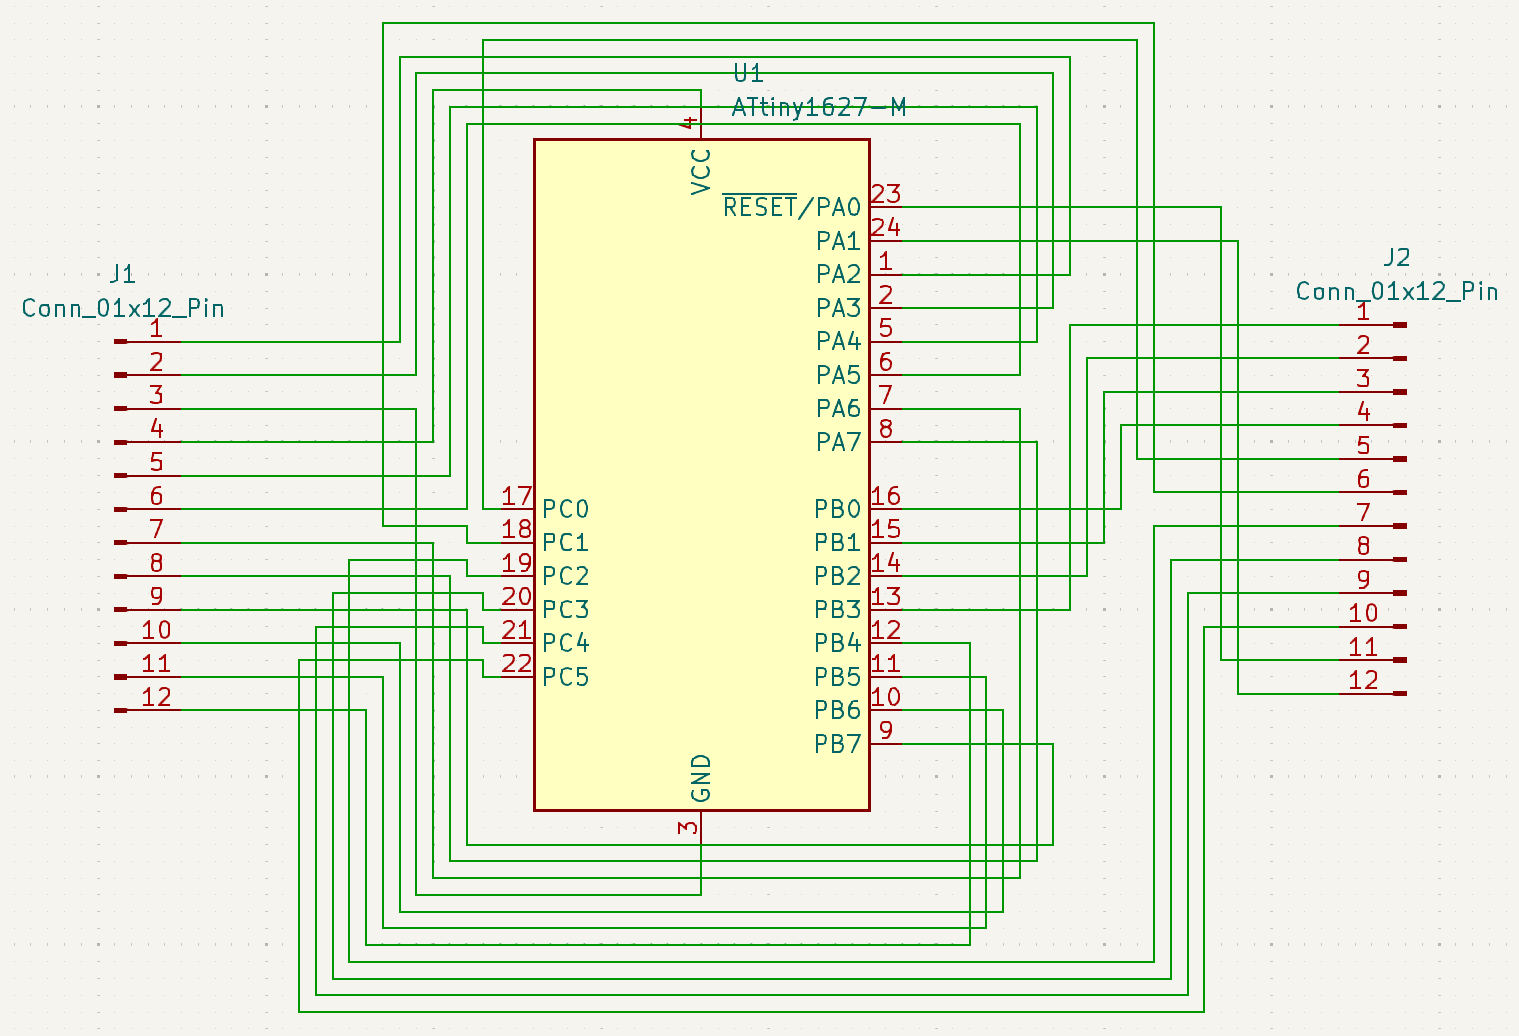
\includegraphics[width= \linewidth]{assets/breakout_schematic.png}
	\end{center}
	\begin{center}
		\label{picture:breakout2}
		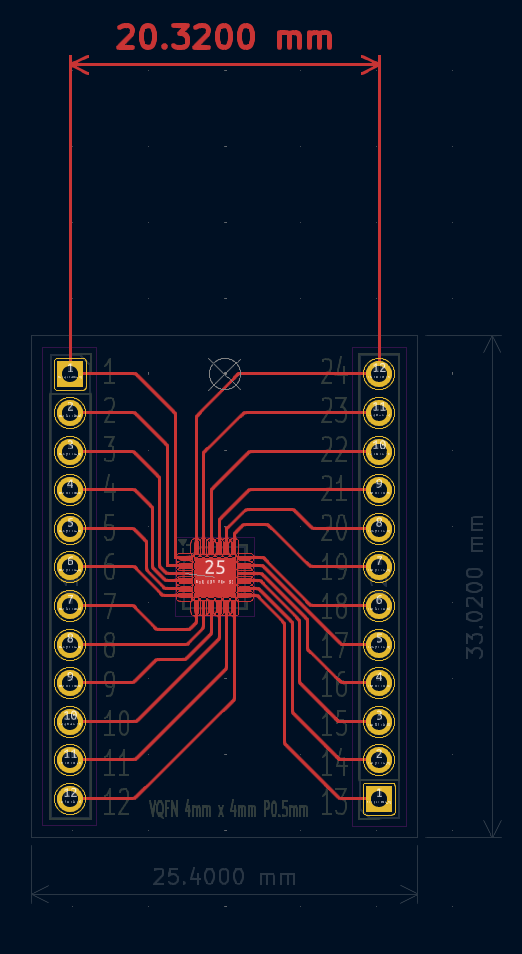
\includegraphics[width= \linewidth]{assets/breakout_pcb_schema.png}
	\end{center}
	\begin{center}
		\label{picture:breakout3}
		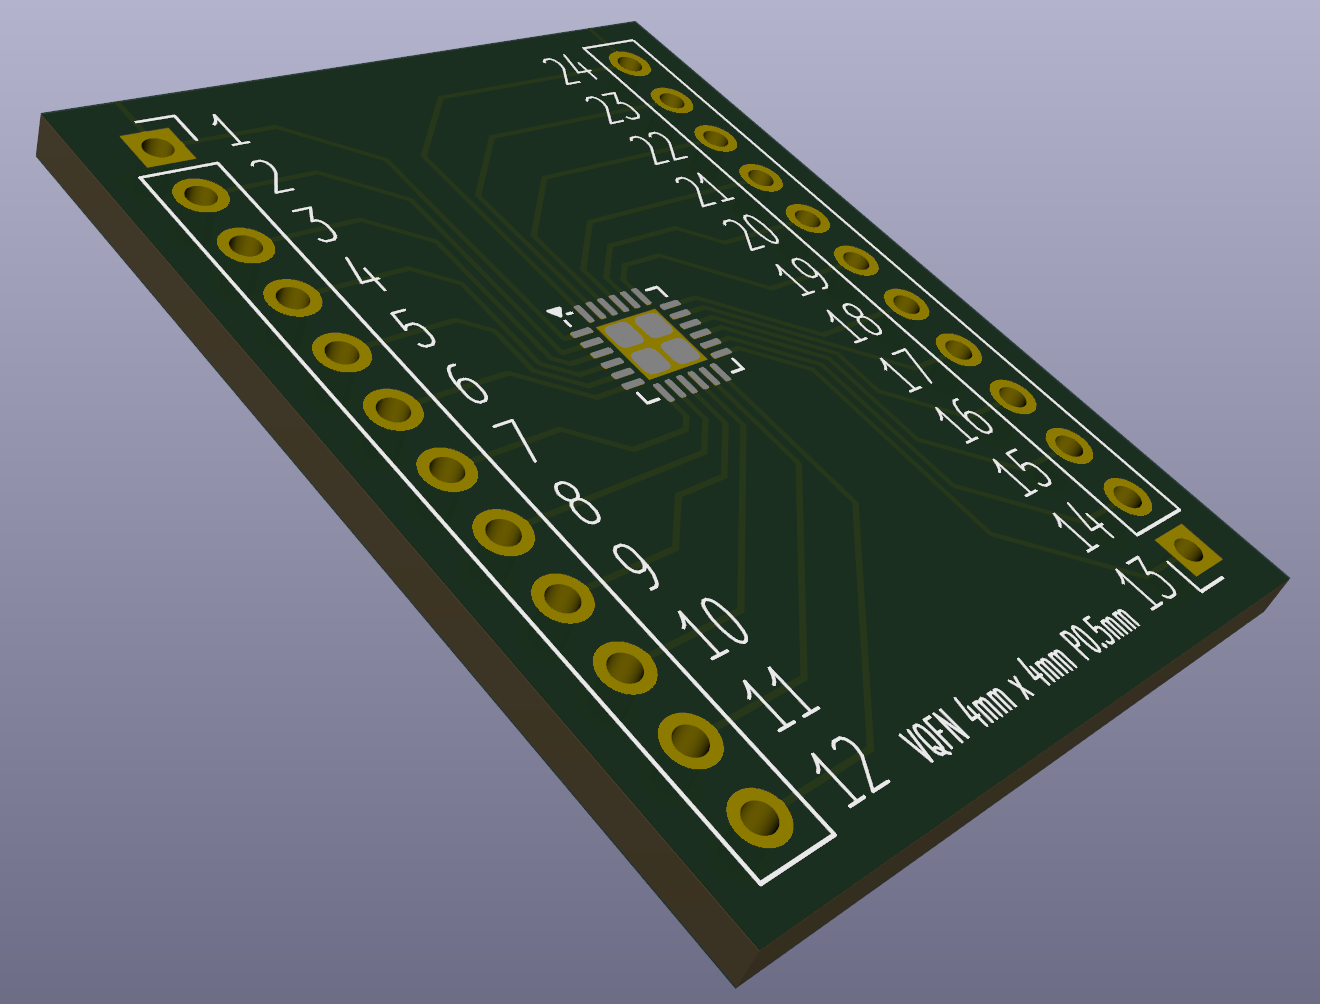
\includegraphics[width= \linewidth]{assets/breakout_pcb_3d.png}
	\end{center}
	
	\section{AUV Electronics Schematics}\label{appendix:auv_electronics_scematics}
	\subsection{AUV Schematic}\label{appendix:auv_schematic}
	\begin{center}
		\label{picture:auv_schematic}
		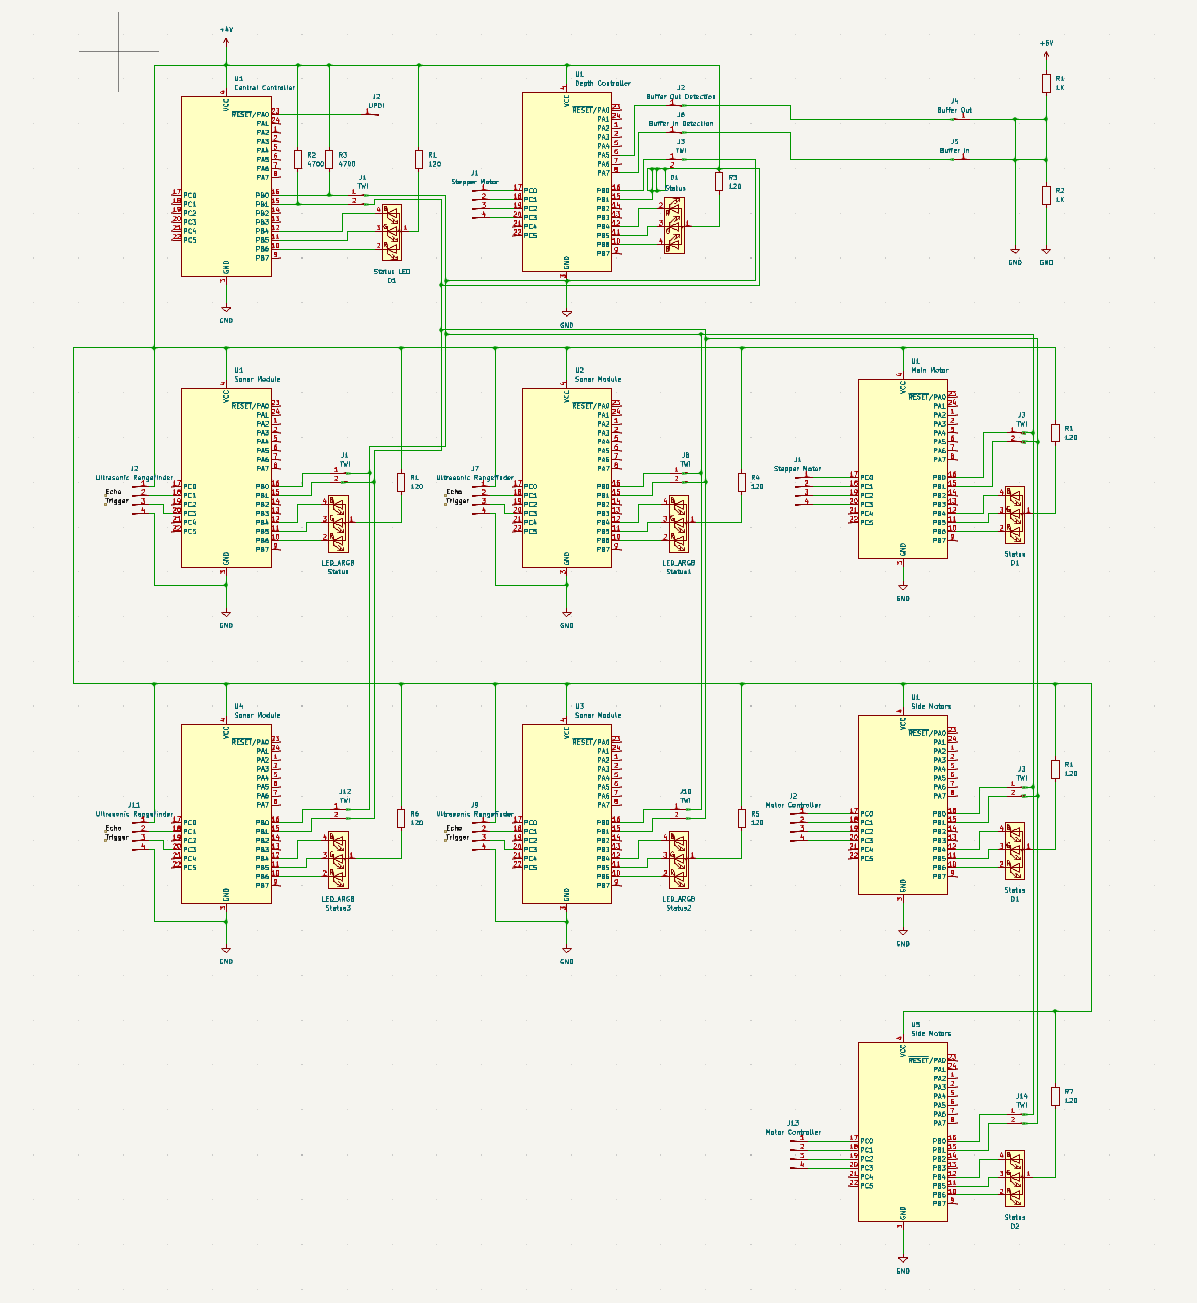
\includegraphics[width=\linewidth]{assets/AUVSchematic.png}
	\end{center}
	\subsection{Central Controller Schematic}\label{appendix:central_controller_schematic}
	\begin{center}
		\label{picture:central_controller_schematic}
		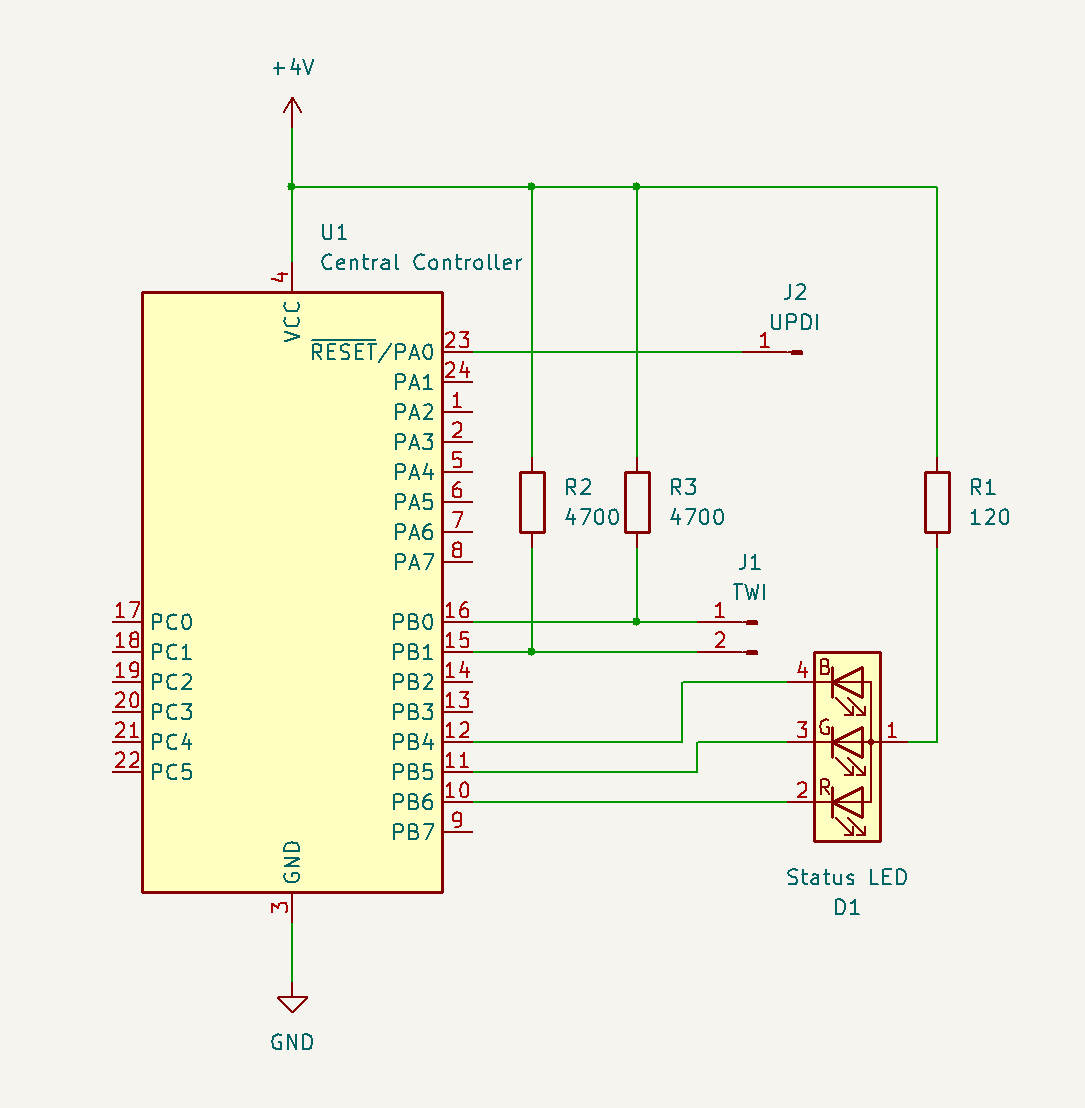
\includegraphics[width=\linewidth]{assets/CentralControllerSchematic.png}
	\end{center}
	\subsection{Depth Controller Schematic}\label{appendix:depth_controller_schematic}
	\begin{center}
		\label{picture:depth_controller_schematic}
		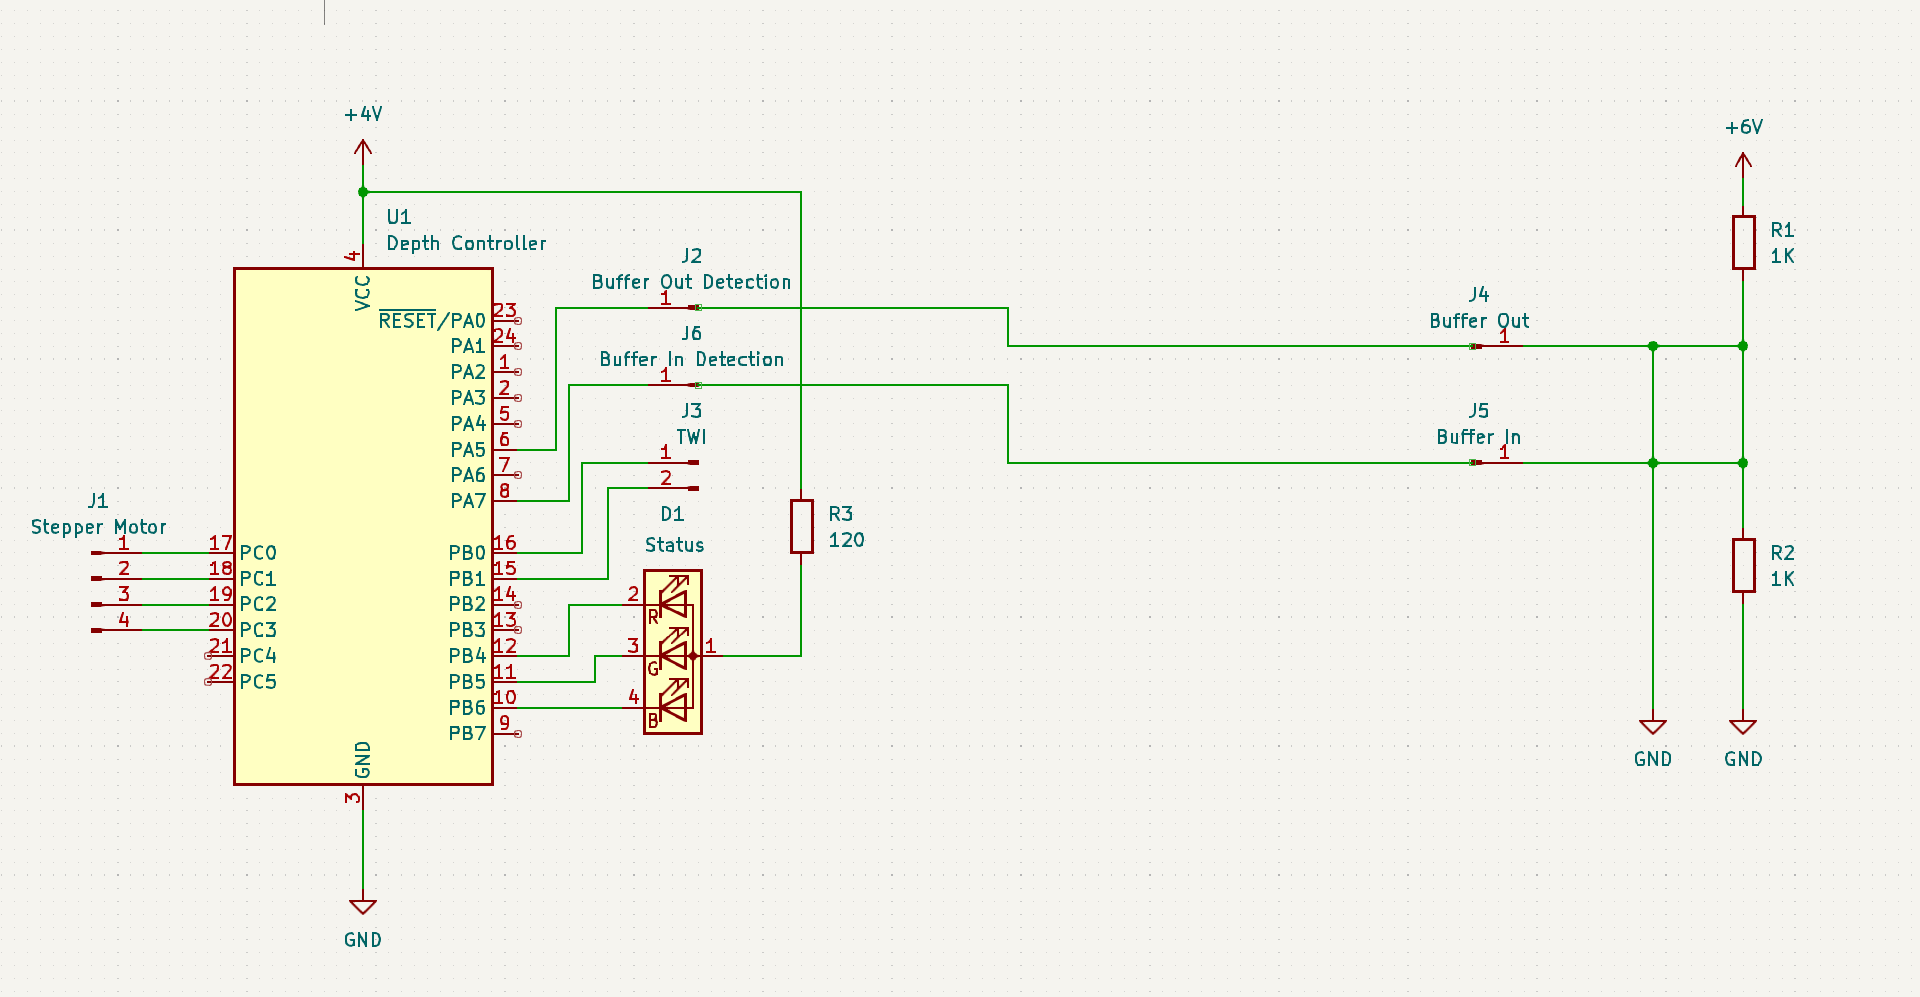
\includegraphics[width=\linewidth]{assets/DepthControllerSchematic.png}
	\end{center}
	\subsection{Sonar Module Schematic}\label{appendix:sonar_schematic}
	\begin{center}
		\label{picture:sonar_schematic}
		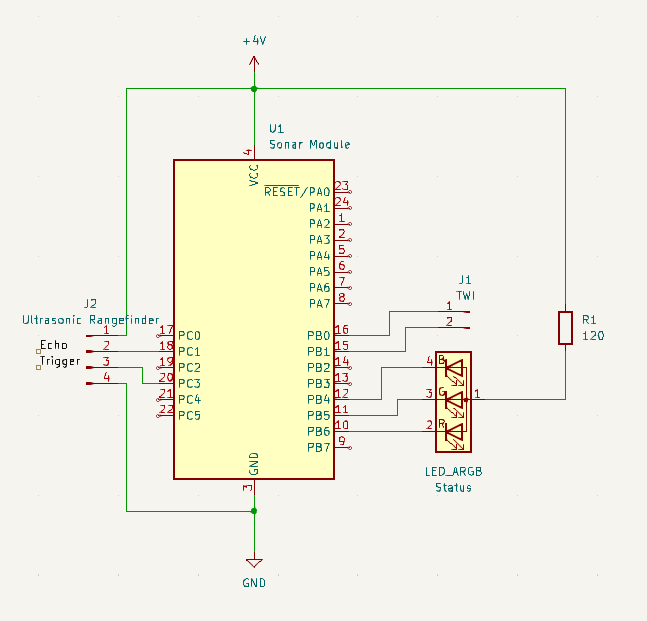
\includegraphics[width=\linewidth]{assets/SonarModuleSchematic.png}
	\end{center}
	\subsection{Main Motor Schematic}\label{appendix:main_motor_schematic}
	\begin{center}
		\label{picture:main_motor_schematic}
		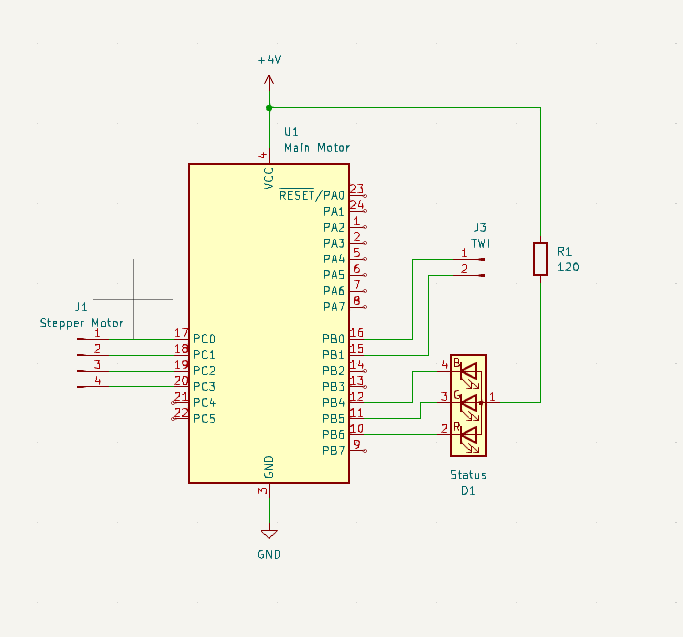
\includegraphics[width=\linewidth]{assets/MainMotorSchematic.png}
	\end{center}
	\subsection{Side Motor Schematic}\label{appendix:side_motor_schematic}
	\begin{center}
		\label{picture:side_motor_schematic}
		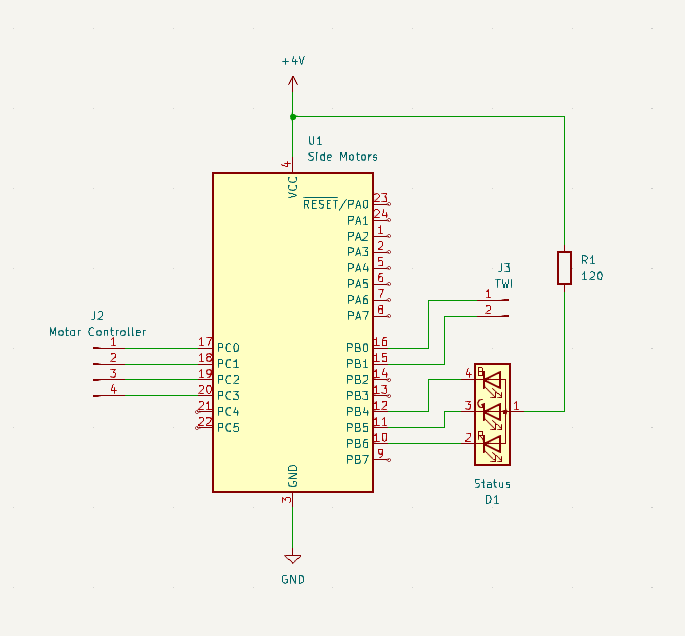
\includegraphics[width=\linewidth]{assets/SideMotorSchematic.png}
	\end{center}
	
	
	
	
	\printbibliography
\end{document}